\documentclass{article}
\usepackage[utf8]{inputenc}
\usepackage{indentfirst}
\usepackage{graphicx}
\usepackage{hyperref}
\hypersetup{
    colorlinks,
    citecolor=black,
    filecolor=black,
    linkcolor=red,
    urlcolor=blue,
}

\title{\textbf{Dimensionality Reduction Report}}
\author{Octave Cinquanta}
\date{November 2021}

\begin{document}

\maketitle

\section{Introduction}

For the course of Dimensionality Reduction, we have been given an artificial dataset containing data on a dating app, such as the users' profile score, their number of matches, number of photos uploaded, etc... We were to use this dataset to learn and practice different analysis and clustering methods, such as Principal Component Analysis, Multiple Correspondence Analysis and k-means clustering.

\section{Identifying correlations in the variables}

\begin{figure}[h]
    \centering
    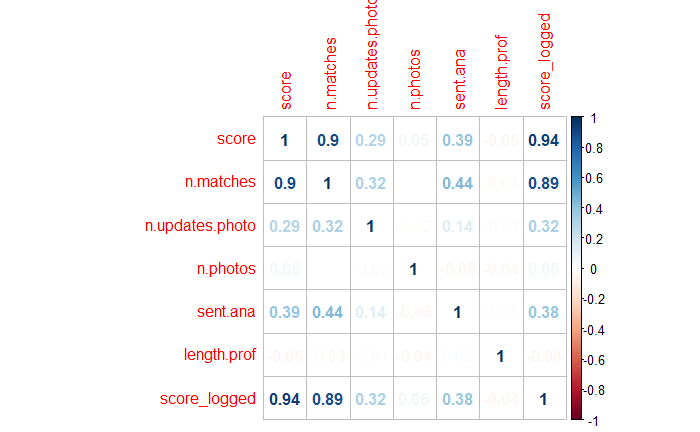
\includegraphics[width=\textwidth]{cor.png}
    \caption{Correlation plot of the numerical variables of users}
    \label{cor}
\end{figure}

We carried out multiple correlation tests between various variables and in the end produced a correlation plot of the numerical variables of the dataset, as seen in \hyperref[cor]{Figure 1}. As we can see there is a very significant correlation between the user's score and their number of matches. There is also a mild correlation between other variables, such as between the number of matches and the sentimental analysis for instance.

\section{Dimensionality Reduction}

\begin{figure}[h]
    \centering
    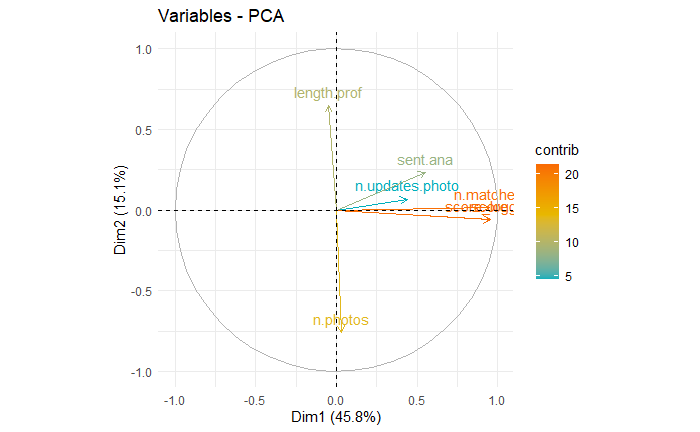
\includegraphics[width=\textwidth]{circle.png}
    \caption{Variable circle of correlations of users}
    \label{circle}
\end{figure}

We used the dataset to produce a variable circle of correlation as seen in \hyperref[circle]{Figure 2}. This circle shows us that the biggest contributors amongst variables are the number of matches and the score. Those variables can be seen as the principal components and could be called the "attractiveness" of the user's profile. We can also see that the sentimental analysis and the number of photo updates have a small contribution to offer, while the length of the profile and the overall number of photos are completely unrelated to the case. \\
We have also produced an \hyperref[ind]{individual map} and a \hyperref[biplot]{biplot} using a sample of individuals. Those plots allow us to have a better look at the contributions on an individual level as well as the previously obtained variable level. We can see that there are much more significant individuals present along the first dimension than the second, and more in the positive than on the negative. 

\begin{figure}[h]
    \centering
    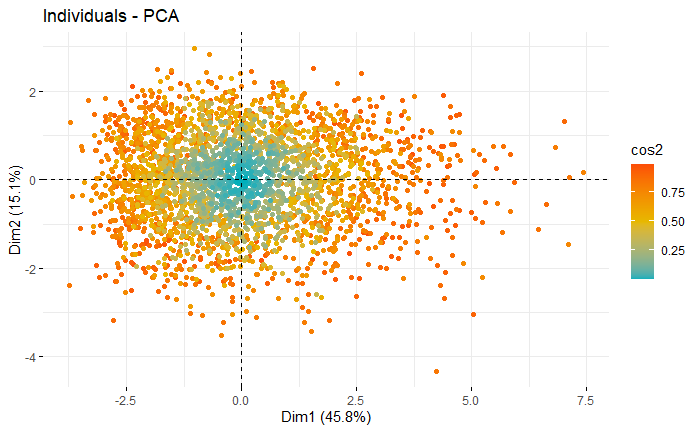
\includegraphics[width=\textwidth]{ind.png}
    \caption{Individual map with a high number of individuals}
    \label{ind}
\end{figure}

\begin{figure}[h!]
    \centering
    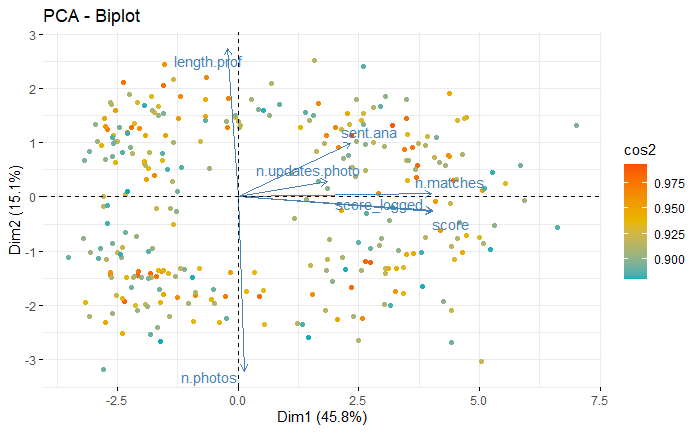
\includegraphics[width=\textwidth]{biplot.png}
    \caption{Biplot with a sample of individuals}
    \label{biplot}
\end{figure}

We have also obtained a table of loadings as we can see in \hyperref[loadings]{Figure 5}. We see that the first component is composed of only a major negative coefficient from the profile length. The second component is composed of a major positive coefficient from the number of matches and a slight positive coefficient from the sentimental analysis. The third component is composed of a major negative coefficient from the sentimental analysis and a slight positive coefficient from the number of photos. The fourth component is composed of a major positive coefficient from the number of photos and a slight positive coefficient from the sentimental analysis. The fifth component is composed of only a major positive coefficient from the number of photo updates. The sixth component is composed of a major positive coefficient from the score, a slight negative coefficient from the number of matches and a slight positive coefficient from the logged score. The seventh component is composed of a slight positive coefficient from the score and a major negative coefficient from the logged score.

\begin{figure}[h]
    \centering
    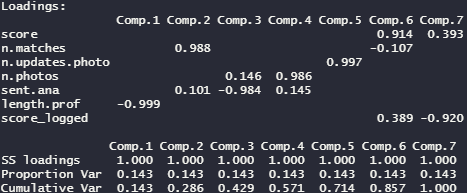
\includegraphics[width=\textwidth]{loadings.png}
    \caption{Table of loadings of the various variables}
    \label{loadings}
\end{figure}

We have performed a Multiple Correspondence Analysis, and produced a plot, \hyperref[mca]{Figure 6}, of the interaction between the variables and the dimensions of the analysis. We can see that the variable gender is the most correlated with dimension 1 and also heavily correlated with dimension 2. Both the voyage and laugh variables are also majorly correlated with dimension 2. The photo.beach variable is quite correlated with dimension 1, and that is also the case with the photo.keke variable.

\begin{figure}[h]
    \centering
    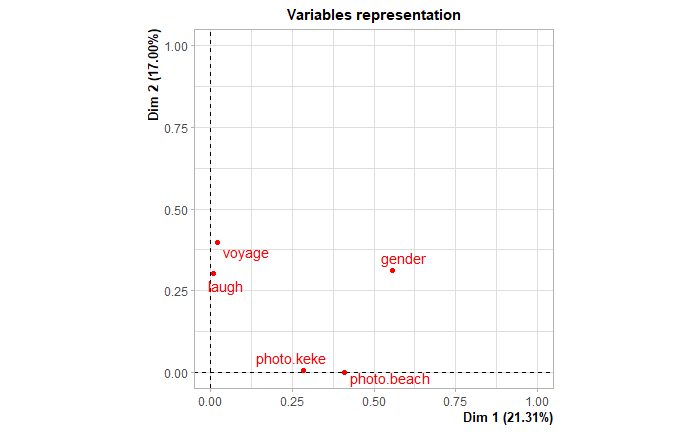
\includegraphics[width=\textwidth]{mca.png}
    \caption{MCA variables plotted}
    \label{mca}
\end{figure}

\section{k-means and Hierarchical Clustering}

The k-means algorithm works as follows: the algorithm picks k random centroids, it then uses Euclidean distance to assign each data point to its nearest centroid, it then moves every centroid to the average of its assigned points, and then it keeps moving the centroids until there is no more movement possible. Those centroids then become the clusters we wish to obtain. \\
In order to choose an appropriate number of clusters, we produced a scree plot of the users, that is \hyperref[scree]{Figure 7}. Looking at the plot, we can notice the elbow of the graph, and we chose to have 5 clusters because of it.

\begin{figure}[h]
    \centering
    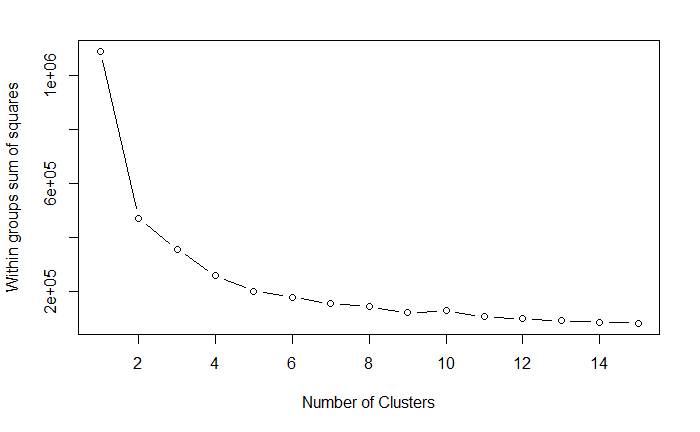
\includegraphics[width=\textwidth]{screeplot.png}
    \caption{Scree plot of the users clusters using sum of squares}
    \label{scree}
\end{figure}

Through k-means clustering, we obtained the results displayed in \hyperref[k]{Figure 8}. We can see that the clusters are very on top of each others and badly defined with poor boundaries between each others. 

\begin{figure}[h]
    \centering
    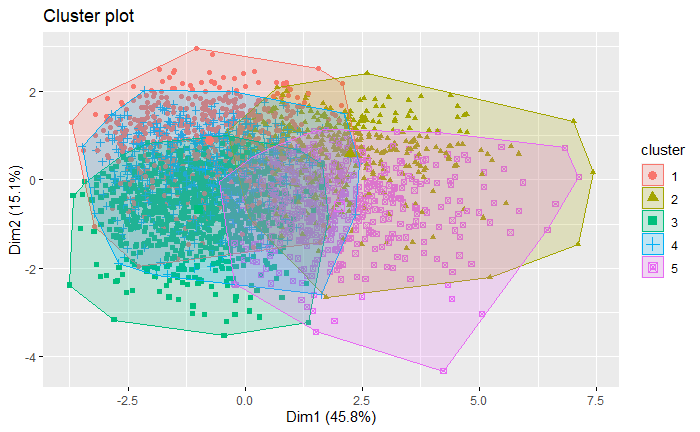
\includegraphics[width=\textwidth]{k.png}
    \caption{Plot of the k-means clusters}
    \label{k}
\end{figure}

The hierarchical clustering algorithm works as follows: it starts off treating every single observation like a cluster, and then merges the clusters with their closest neighbour one by one until there is only a single cluster left. The algorithm retains all those operations and transforms them into a dendogram, a tree-like plot that operates in the opposite as its algorithm: it shows one big cluster dividing itself into several and then into the observations themselves. \\
k-means and hierarchical clustering both have their own pros and cons, such as:
\begin{itemize}
    \item It is easier to determine the number of clusters using the Hierarchical Clustering
    \item The results of HC are more easily readable and interpreted
    \item But the k-means algorithm runs faster
    \item And it is better to use k-means if we already the number of clusters
\end{itemize}
In the end, choosing which algorithm to use depends heavily on the data we have, but if time allows it trying to use both might not be a bad idea either. 

\begin{figure}[h]
    \centering
    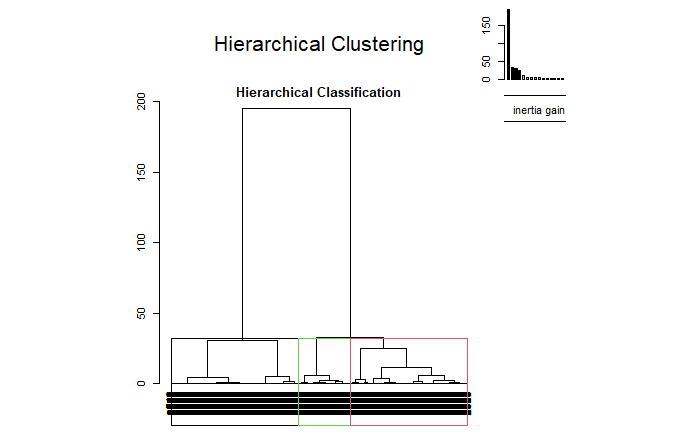
\includegraphics[width=\textwidth]{dend.png}
    \caption{Dendogram of the HC clusters}
    \label{dend}
\end{figure}

\begin{figure}[h]
    \centering
    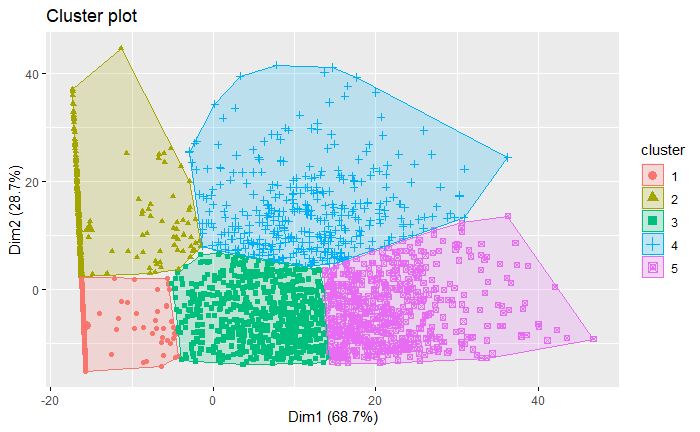
\includegraphics[width=\textwidth]{hc.png}
    \caption{Plot of the Hierarchical Clustering clusters}
    \label{hc}
\end{figure}

We can have a look at the results provided by the Hierarchical Clustering through \hyperref[dend]{Figure 9}, the dendogram we obtained, and the plot of the clusters, \hyperref[hc]{Figure 10}. We can see that the clusters are not overlapping like the k-means, they are rather clear-cut. The cluster plot does indicate a much better dimensional representation through the Hierarchical Clustering, and it was as such the much more successful clustering method of the two.

\end{document}
